\documentclass[11pt]{scrartcl}
\usepackage[usenames,dvipsnames,svgnames]{xcolor}
\usepackage[shortlabels]{enumitem}
\usepackage[framemethod=TikZ]{mdframed}
\usepackage{amsmath,amssymb,amsthm}
\usepackage{epigraph}
\usepackage[colorlinks]{hyperref}
\usepackage{microtype}
\usepackage{mathtools}
\usepackage[headsepline]{scrlayer-scrpage}
\usepackage{thmtools}
\usepackage{listings}
\usepackage{derivative}
\renewcommand{\epigraphsize}{\scriptsize}
\renewcommand{\epigraphwidth}{60ex}
\addtolength{\textheight}{3.14cm}
\ihead{\footnotesize\textbf{DGW-elemgeo}}
\ohead{\footnotesize Updated Fri 30 Aug 2024 13:58:12 UTC}
\providecommand{\clubs}[1]{$#1\clubsuit$}
\providecommand{\clubg}[1]{\bgroup\color{green!40!black}[$#1\clubsuit$]\egroup}

\providecommand{\ol}{\overline}
\providecommand{\eps}{\varepsilon}
\providecommand{\half}{\frac{1}{2}}
\providecommand{\dang}{\measuredangle} %% Directed angle
\providecommand{\CC}{\mathbb C}
\providecommand{\FF}{\mathbb F}
\providecommand{\NN}{\mathbb N}
\providecommand{\QQ}{\mathbb Q}
\providecommand{\RR}{\mathbb R}
\providecommand{\ZZ}{\mathbb Z}
\providecommand{\dg}{^\circ}
\providecommand{\ii}{\item}
\providecommand{\alert}{\textbf}
\providecommand{\opname}{\operatorname}
\providecommand{\ts}{\textsuperscript}
% hacks for arc
\providecommand{\tarc}{\mbox{\large$\frown$}}
\providecommand{\arc}[1]{\stackrel{\tarc}{#1}}
\reversemarginpar
\providecommand{\printpuid}[1]{\marginpar{\href{https://otis.evanchen.cc/arch/#1}{\ttfamily\footnotesize\color{green!40!black}#1}}}

\mdfdefinestyle{mdbluebox}{roundcorner=10pt,innerbottommargin=9pt,
    linecolor=blue,backgroundcolor=TealBlue!5,}
\declaretheoremstyle[headfont=\sffamily\bfseries\color{MidnightBlue},
    mdframed={style=mdbluebox},]{thmbluebox}
\mdfdefinestyle{mdredbox}{frametitlefont=\bfseries,innerbottommargin=8pt,
    nobreak=true,backgroundcolor=Salmon!5,linecolor=RawSienna,}
\declaretheoremstyle[headfont=\bfseries\color{RawSienna},
    mdframed={style=mdredbox},headpunct={\\[3pt]},postheadspace=0pt,]{thmredbox}
\mdfdefinestyle{mdgreenbox}{linecolor=ForestGreen,backgroundcolor=ForestGreen!5,
    linewidth=2pt,rightline=false,leftline=true,topline=false,bottomline=false,}
\declaretheoremstyle[headfont=\bfseries\sffamily\color{ForestGreen!70!black},
    mdframed={style=mdgreenbox},headpunct={ --- },]{thmgreenbox}
\mdfdefinestyle{mdblackbox}{linecolor=black,backgroundcolor=RedViolet!5!gray!5,
    linewidth=3pt,rightline=false,leftline=true,topline=false,bottomline=false,}
\declaretheoremstyle[mdframed={style=mdblackbox}]{thmblackbox}
\declaretheorem[style=thmredbox,name=Problem]{problem}
\declaretheorem[style=thmredbox,name=Required Problem,sibling=problem]{reqproblem}
\declaretheorem[style=thmbluebox,name=Theorem,numberwithin=problem]{theorem}
\declaretheorem[style=thmbluebox,name=Lemma,sibling=theorem]{lemma}
\declaretheorem[style=thmbluebox,name=Theorem,numbered=no]{theorem*}
\declaretheorem[style=thmbluebox,name=Lemma,numbered=no]{lemma*}
\declaretheorem[style=thmgreenbox,name=Claim,sibling=theorem]{claim}
\declaretheorem[style=thmgreenbox,name=Claim,numbered=no]{claim*}
\declaretheorem[style=thmblackbox,name=Remark,sibling=theorem]{remark}
\declaretheorem[style=thmblackbox,name=Remark,numbered=no]{remark*}
\declaretheorem[style=thmgreenbox,name=Definition,sibling=theorem]{definition}
\declaretheorem[style=thmgreenbox,name=Definition,numbered=no]{definition*}
\declaretheorem[style=thmblackbox,name=Example,sibling=theorem]{example}
\declaretheorem[style=thmblackbox,name=Example,numbered=no]{example*}

\newenvironment{walkthrough}{\noindent\textbf{\color{green!40!black}Walkthrough.}}{}
\newlist{walk}{enumerate}{3}
\setlist[walk]{label=\bfseries (\alph*)}

\usepackage{asymptote}
\begin{asydef}
size(8cm); // set a reasonable default
usepackage("amsmath");
usepackage("amssymb");
settings.tex="pdflatex";
settings.outformat="pdf";
import geometry;
void filldraw(picture pic = currentpicture, conic g, pen fillpen=defaultpen, pen drawpen=defaultpen) { filldraw(pic, (path) g, fillpen, drawpen); }
void fill(picture pic = currentpicture, conic g, pen p=defaultpen) { filldraw(pic, (path) g, p); }
pair foot(pair P, pair A, pair B) { return foot(triangle(A,B,P).VC); }
pair centroid(pair A, pair B, pair C) { return (A+B+C)/3; }
\end{asydef}

\newcommand{\goals}[2]{\bgroup
\sffamily\small \emph{Instructions}: Solve \clubg{#1}.
If you have time, solve \clubg{#2}.\egroup\par}

%% 426c616e6b204c615465587e
\begin{document}
\title{Submission for DGW-ELEMGEO}
\subtitle{OTIS (internal use)}
\author{Michael Middlezong}
\date{\today}
\maketitle

\begin{example*}[Monge's theorem, $0\clubsuit$]
  Let $\omega_1$, $\omega_2$, $\omega_3$ be three pairwise incongruent circles,
  and let $X_{12}$, $X_{23}$, $X_{31}$ be the pairwise exsimilicenters.
  Show that $X_{12}$, $X_{23}$, $X_{31}$ are collinear.
  \begin{center}
  \begin{asy}
  size(8cm);
  pair A = (1.4,3);
  pair B = (0,0);
  pair C = (4,0);
  real a = 1.7;
  real b = 0.5;
  real c = 0.8;
  filldraw(circle(A,a), paleyellow, black+2);
  filldraw(circle(B,b), paleyellow, black+2);
  filldraw(circle(C,c), paleyellow, black+2);
  pair X = b/(b-c)*(C-B)+B;
  pair Y = c/(c-a)*(A-C)+C;
  pair Z = a/(a-b)*(B-A)+A;
  dot("$X_{23}$", X, dir(270));
  dot("$X_{31}$", Y, dir(270));
  dot("$X_{12}$", Z, dir(270));
  draw(X--Y, dashed+red);
  void draw_tangents(pair P, pair O, real r) {
  pair Q = r*r / conj(P-O) + O;
  pair R = dir(P-O)*dir(90) + Q;
  path l = (9*Q-8*R)--(9*R-8*Q);
  pair T1 = intersectionpoints(l,circle(O,r))[0];
  pair T2 = intersectionpoints(l,circle(O,r))[1];
  draw(T1--P--T2, deepblue);
  }
  draw_tangents(Y,A,a);
  draw_tangents(Z,A,a);
  draw_tangents(X,C,c);
  label("$\omega_1$", A);
  label("$\omega_2$", B);
  label("$\omega_3$", C);
  \end{asy}
  \end{center}
\end{example*} \printpuid{ZABF24E3}

\begin{walkthrough}
Let $h_{12}$ denote the homothety sending $\omega_1$ to $\omega_2$,
which is a function from the plane to itself.
Define $h_{23}$ and $h_{13}$ similarly.
\begin{walk}
  \ii The function composition $h_{23} \circ h_{12}$ is a homothety too.
  Which is it?
  \ii Show that $h_{13}(X_{12})$ is collinear with $X_{12}$ and $X_{31}$.
  \ii Show that $h_{23}(X_{12})$ is collinear with $X_{12}$ and $X_{23}$.
  \ii Conclude.
\end{walk}
\end{walkthrough}
%% You're not expected to write up walkthroughs (unless you really want to).
%% The source is just for your reference.

\begin{example*}[\href{https://aops.com/community/p23524100}{USEMO 2021/4, Sayandeep Shee}, $0\clubsuit$]
  Let $ABC$ be a triangle with circumcircle $\omega$,
  and let $X$ be the reflection of $A$ in $B$.
  Line $CX$ meets $\omega$ again at $D$.
  Lines $BD$ and $AC$ meet at $E$, and lines $AD$ and $BC$ meet at $F$.
  Let $M$ and $N$ denote the midpoints of $AB$ and $AC$.

  Can line $EF$ share a point with the circumcircle of triangle $AMN$?
\end{example*} \printpuid{21USEMO4}

\begin{walkthrough}
There are lots of different approaches.
We'll give the most classical one presented by the author,
but there are plenty of other things that could work too!
\begin{walk}
  \ii Let $P$ be the midpoint of $\ol{AD}$.
  Where else does $P$ lie?
  \ii Show that $FB^2 = FP \cdot FA$.
  \ii Show that $EB^2 = EN \cdot EA$.
  \ii Using radical axis with a circle of radius zero at $B$,
  prove that line $EF$ is disjoint from $(AMN)$.
\end{walk}
\end{walkthrough}
%% You're not expected to write up walkthroughs (unless you really want to).
%% The source is just for your reference.

\begin{example*}[\href{https://aops.com/community/p10226149}{JMO 2018/3, Ray Li}, $0\clubsuit$]
  Let $ABCD$ be a quadrilateral inscribed
  in circle $\omega$ with $\ol{AC} \perp \ol{BD}$.
  Let $E$ and $F$ be the reflections of $D$ over
  $\ol{BA}$ and $\ol{BC}$, respectively, and let $P$ be
  the intersection of $\ol{BD}$ and $\ol{EF}$.
  Suppose that the circumcircles of $EPD$ and $FPD$
  meet $\omega$ at $Q$ and $R$ different from $D$.
  Show that $EQ = FR$.
\end{example*} \printpuid{18JMO3}

\begin{walkthrough}
Most of this problem is about realizing where
the points $P$, $Q$, $R$ are.
\begin{walk}
  \ii Using what you know about the Simson line,
  figure out where point $P$ is.
  \ii Determine the circumcenters of
  $\triangle EPD$ and $\triangle FPD$.
  \ii Figure out where the points $Q$ and $R$ are.
  \ii Finish the problem.
\end{walk}
\end{walkthrough}
%% You're not expected to write up walkthroughs (unless you really want to).
%% The source is just for your reference.

\begin{example*}[\href{https://aops.com/community/p8526136}{TSTST 2017/5, Ray Li}, $0\clubsuit$]
  Let $ABC$ be a triangle with incenter $I$.
  Let $D$ be a point on side $BC$ and let $\omega_B$ and $\omega_C$
  be the incircles of $\triangle ABD$ and $\triangle ACD$, respectively.
  Suppose that $\omega_B$ and $\omega_C$ are tangent to segment $BC$
  at points $E$ and $F$, respectively.
  Let $P$ be the intersection of segment $AD$ with the
  line joining the centers of $\omega_B$ and $\omega_C$.
  Let $X$ be the intersection point of lines $BI$ and $CP$
  and let $Y$ be the intersection point of lines $CI$ and $BP$.
  Prove that lines $EX$ and $FY$ meet on the incircle of $\triangle ABC$.
\end{example*} \printpuid{17TSTST5}

\begin{walkthrough}
%%fakesection Walkthrough
Let $\omega$ denote the incircle of $\triangle ABC$.
\begin{walk}
  \ii Identify the point $Z = \ol{EX} \cap \ol{FY}$ in a good diagram.
  (This was worth a point! Despite this, many contestants were unable to find it.)
  \ii Consider the positive homothety sending $\omega$ to $\omega_C$.
  Determine its center.
  \ii Consider the negative homothety sending $\omega_C$ to $\omega_B$.
  Determine its center.
  \ii The composition of the previous two homotheties
  in (b) and (c) is a negative homothety
  sending $\omega$ to $\omega_B$.
  Determine with proof the center of this homothety.

  This is not as simple as the previous two parts;
  you will need to \emph{use} (b) and (c) to do this part,
  as well as the simple observation that the center
  should lie on the $\angle B$ bisector.
  \ii Conclude that $\ol{FY}$ passes through the point you claimed in (a).
\end{walk}
Experts may notice that this walkthrough gives what is essentially
a proof of Monge d'Alembert theorem.
\end{walkthrough}
%% You're not expected to write up walkthroughs (unless you really want to).
%% The source is just for your reference.

\begin{example*}[\href{https://aops.com/community/p6575204}{TSTST 2016/2, Evan Chen}, $0\clubsuit$]
  Let $ABC$ be a scalene triangle with orthocenter $H$ and circumcenter $O$
  and denote by $M$, $N$ the midpoints of $\ol{AH}$, $\ol{BC}$.
  Suppose the circle $\gamma$ with diameter $\ol{AH}$ meets
  the circumcircle of $ABC$ at $G \neq A$,
  and meets line $\ol{AN}$ at $Q \neq A$.
  The tangent to $\gamma$ at $G$ meets line $OM$ at $P$.
  Show that the circumcircles of $\triangle GNQ$
  and $\triangle MBC$ intersect on $\ol{PN}$.
\end{example*} \printpuid{16TSTST2}

\begin{walkthrough}
%%fakesection Walkthrough
Let $DEF$ be the orthic triangle of $ABC$.
\begin{walk}
  \ii Show that $P$ is really just the intersection
  of the tangents to $\gamma$ at $A$ and $G$
  (and thus the line $\ol{OM}$ is just a distraction).
  \ii Show that lines $\ol{AG}$, $\ol{EF}$, $\ol{BC}$ are concurrent, say at $R$.
  \ii Prove that $(PAMG)$, $(MBC)$, $(MFDNE)$ are concurrent at a point $T \neq M$.
  \ii Show that $T = \ol{PN} \cap \ol{MR}$.
  \ii Show that $R \in \ol{HQ}$.
  \ii Show that $R$, $G$, $T$, $Q$, $N$ are concyclic, completing the proof.
\end{walk}
\end{walkthrough}
%% You're not expected to write up walkthroughs (unless you really want to).
%% The source is just for your reference.

\newpage

% ========================================
\section*{Practice problems}
\goals{42}{56}

\epigraph{Life is full of surprises, but never when you need one.}
{Calvin in \emph{Calvin and Hobbes}}

\begin{problem}[\href{https://aops.com/community/p5083627}{India TST 2015/1}, $3\clubsuit$]
  Diagonals $\ol{AC}$ and $\ol{BD}$ of convex quadrilateral $ABCD$ meet at $P$.
  Prove that the incenters of the triangles
  $\triangle PAB$, $\triangle PBC$, $\triangle PCD$, $\triangle PDA$
  are concyclic if and only if their $P$-excenters are also concyclic.
\end{problem} \printpuid{15INDTST1}

%% Type your solution to India TST 2015/1 (\href{https://otis.evanchen.cc/arch/15INDTST1/}{15INDTST1}) here ...

%% --------------------------------------------------

\begin{problem}[Added by Atul Shatavart Nadig, $3\clubsuit$]
  Let $ABC$ be a triangle with $\angle A = 120\dg$.
  The angle bisectors of $ABC$ meet the opposite sides
  at $A_1$, $B_1$, $C_1$.
  Find the measure of $\angle B_1A_1C_1$.
\end{problem} \printpuid{Z284BC3E}

%% Type your solution to Added by Atul Shatavart Nadig (\href{https://otis.evanchen.cc/arch/Z284BC3E/}{Z284BC3E}) here ...

%% --------------------------------------------------

\begin{problem}[\href{https://aops.com/community/p14282108}{Iran TST 2020, added by Leonardo Wang}, $2\clubsuit$]
  Let $ABC$ be an isosceles triangle with $AB=AC$ and incenter $I$.
  Circle $\omega$ passes through $C$ and $I$ and is tangent to $AI$.
  Circle $\omega$ intersects $AC$ and circumcircle of $ABC$ at $Q$ and $D$,
  respectively.
  Let $M$ be the midpoint of $AB$ and $N$ be the midpoint of $CQ$.
  Prove that $AD$, $MN$ and $BC$ are concurrent.
\end{problem} \printpuid{20IRNTST10}

%% Type your solution to Iran TST 2020, added by Leonardo Wang (\href{https://otis.evanchen.cc/arch/20IRNTST10/}{20IRNTST10}) here ...

%% --------------------------------------------------

\begin{problem}[\href{https://aops.com/community/p25627509}{Shortlist 2021 G1}, $5\clubsuit$]
  Let $ABCD$ be a parallelogram with $AC=BC$.
  A point $P$ is chosen on the extension of ray $AB$ past $B$.
  The circumcircle of triangle $ACD$ meets the segment $PD$ again at $Q$.
  The circumcircle of triangle $APQ$ meets the segment $PC$ at $R$.
  Prove that lines $CD$, $AQ$, $BR$ are concurrent.
\end{problem} \printpuid{21SLG1}

%% Type your solution to Shortlist 2021 G1 (\href{https://otis.evanchen.cc/arch/21SLG1/}{21SLG1}) here ...

%% --------------------------------------------------

\begin{reqproblem}[\href{https://aops.com/community/p354110}{IMO 2000/1}, $3\clubsuit$]
  Two circles $G_1$ and $G_2$ intersect at two points $M$ and $N$.
  Let $AB$ be the line tangent to these circles at $A$ and $B$,
  respectively, so that $M$ lies closer to $AB$ than $N$.
  Let $CD$ be the line parallel to $AB$
  and passing through the point $M$,
  with $C$ on $G_1$ and $D$ on $G_2$.
  Lines $AC$ and $BD$ meet at $E$; lines $AN$ and $CD$ meet at $P$;
  lines $BN$ and $CD$ meet at $Q$.
  Show that $EP = EQ$.
\end{reqproblem} \printpuid{00IMO1}

%% Type your solution to IMO 2000/1 (\href{https://otis.evanchen.cc/arch/00IMO1/}{00IMO1}), proposed by Sergei Berlov (RUS) here ...
Considering a homothety at $N$ taking $PQ$ to $AB$.
The point $M$ is taken to the midpoint of $AB$ by radical axis,
so thus, $M$ is the midpoint of $PQ$.

It then suffices to show that $EM \perp CD$.
Draw radii from the centers of the circles to the tangency points.
Then, we see that $CD = 2AB$, and the desired result shortly follows.
%% --------------------------------------------------

\begin{problem}[\href{https://aops.com/community/p469044}{APMO 2000/3}, $3\clubsuit$]
  Let $ABC$ be a triangle. Let $M$ and $N$ be the points in which
  the median and the angle bisector,
  respectively, at $A$ meet the side $BC$.
  Let $Q$ and $P$ be the points in which the perpendicular
  at $N$ to $NA$ meets $\ol{MA}$ and $\ol{BA}$, respectively.
  Let $O$ be the point in which the perpendicular at $P$
  to $BA$ meets ray $AN$.
  Prove that $\ol{QO} \perp \ol{BC}$.
\end{problem} \printpuid{00APMO3}

%% Type your solution to APMO 2000/3 (\href{https://otis.evanchen.cc/arch/00APMO3/}{00APMO3}) here ...

%% --------------------------------------------------

\begin{problem}[\href{https://aops.com/community/p15307}{APMO 2004/2}, $2\clubsuit$]
  Let $O$ be the circumcenter and $H$ the orthocenter
  of an acute triangle $ABC$.
  Prove that the area of one of the
  triangles $AOH$, $BOH$ and $COH$ is equal to the
  sum of the areas of the other two.
\end{problem} \printpuid{04APMO2}

%% Type your solution to APMO 2004/2 (\href{https://otis.evanchen.cc/arch/04APMO2/}{04APMO2}) here ...
\begin{center}
    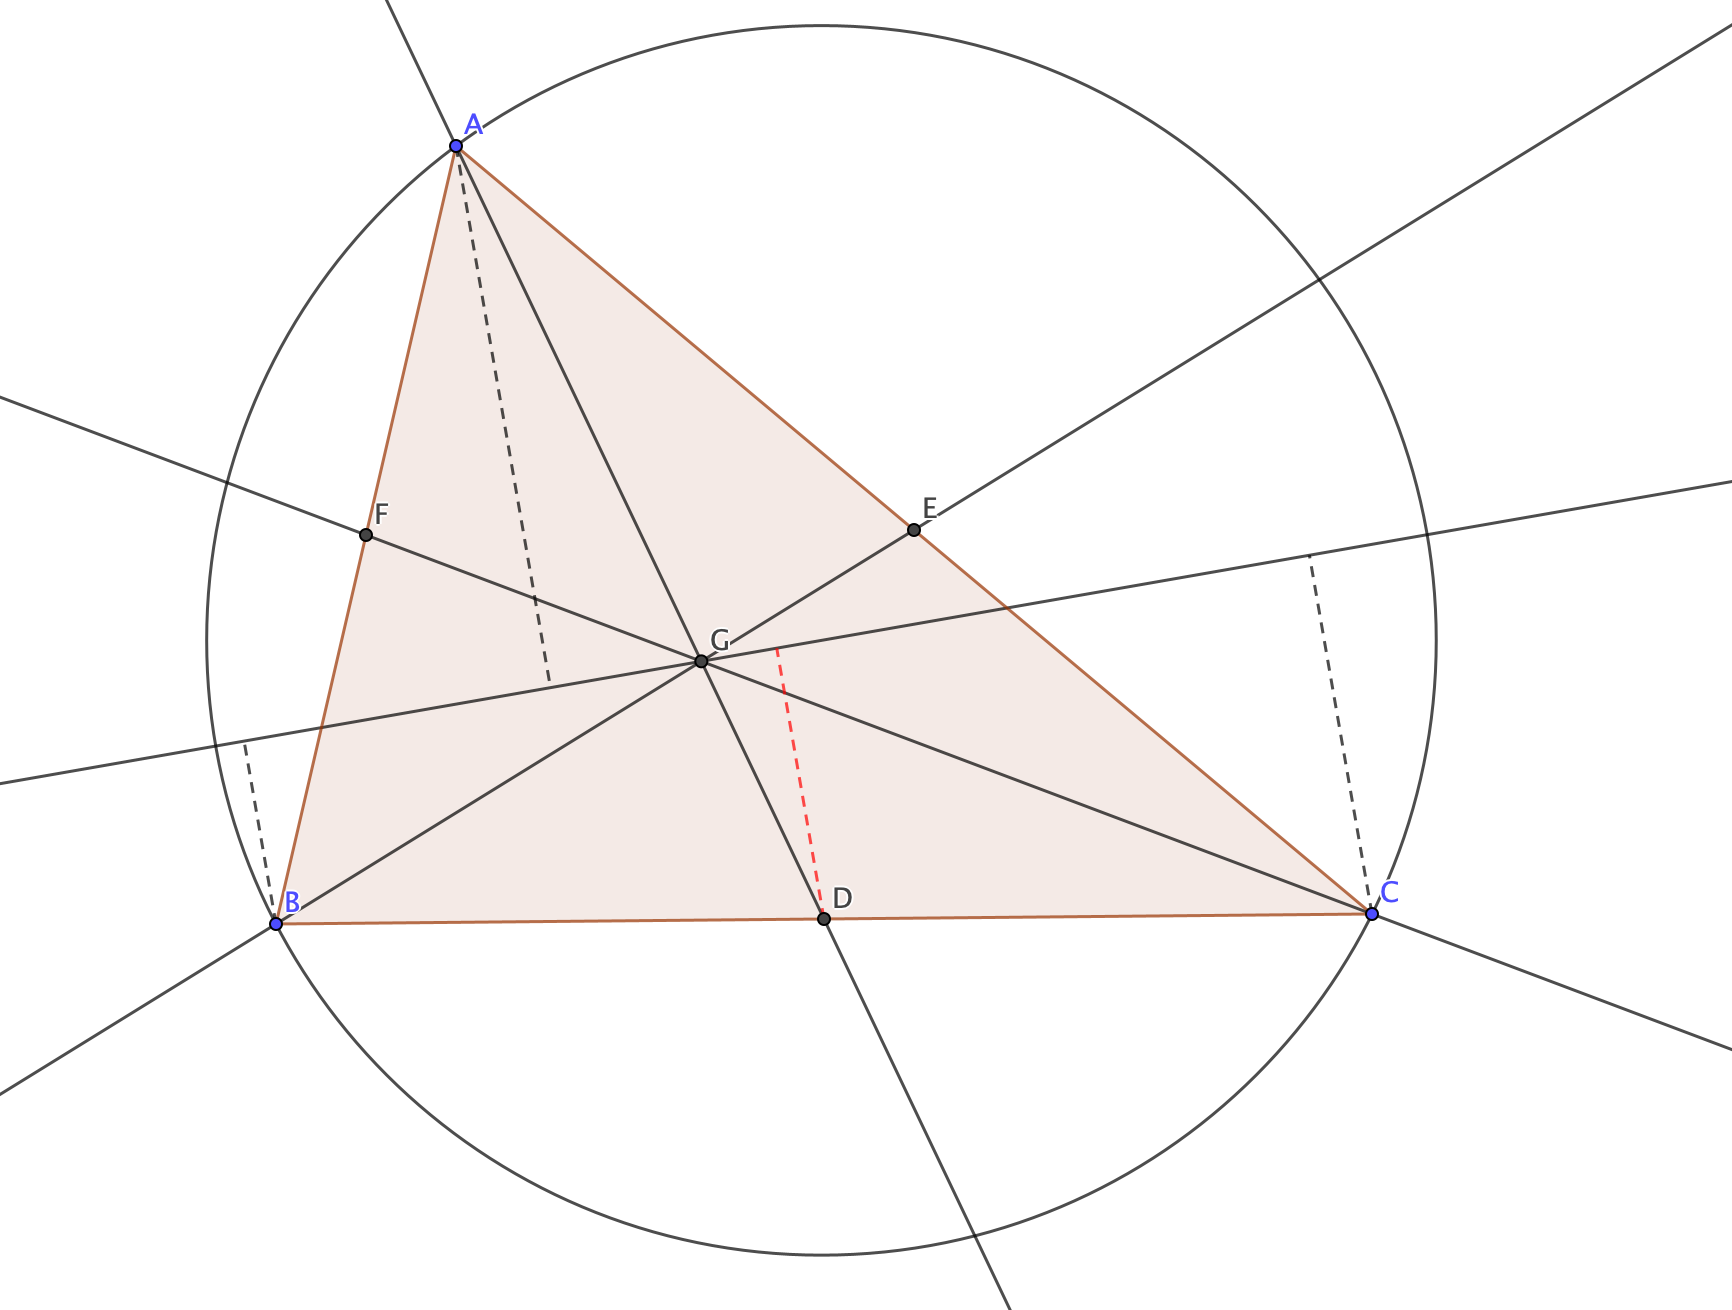
\includegraphics[width=12cm]{04APMO2.png}
\end{center}

Note that line $OH$ passes through $G$, so it suffices to prove
the stronger statement that this works for any line $l$ passing through $G$.

WLOG assume $A$ is on one side of $l$, while $B$ and $C$ are on the other side.
Then, consider a homothety at $G$ with scale factor $-\frac12$.
The distance from $A$ to $l$ is transformed into the distance from
$D$ to $l$, which is clearly the average of the
distance from $B$ to $l$ and the distance from $C$ to $l$,
so we are done.
%% --------------------------------------------------

\begin{problem}[\href{https://aops.com/community/p19116372}{China 2021/4, added by Leonardo Wang}, $5\clubsuit$]
  In acute triangle $ABC$ with $AB > AC$,
  point $M$ is the midpoint of minor arc $BC$,
  $O$ is the circumcenter of $(ABC)$ and $AK$ is its diameter.
  The line parallel to $AM$ through $O$ meets segment $AB$ at $D$,
  and $CA$ extended at $E$.
  Lines $BM$ and $CK$ meet at $P$,
  lines $BK$ and $CM$ meet at $Q$.
  Prove that $\angle OPB+\angle OEB =\angle OQC+\angle ODC$.
\end{problem} \printpuid{21CHN4}

%% Type your solution to China 2021/4, added by Leonardo Wang (\href{https://otis.evanchen.cc/arch/21CHN4/}{21CHN4}) here ...

%% --------------------------------------------------

\begin{problem}[Germany 2015, added by Joel Gerlach, $2\clubsuit$]
  Fix a real number $\ell > 0$ and two rays in the plane with common endpoint $S$.
  Point $A$ moves along one ray, while point $B$ moves along the other ray,
  such that $AS + SB = \ell$.
  Prove that the perpendicular bisector of $AB$
  passes through a fixed point in the plane.
\end{problem} \printpuid{15GER36}

%% Type your solution to Germany 2015, added by Joel Gerlach (\href{https://otis.evanchen.cc/arch/15GER36/}{15GER36}) here ...

%% --------------------------------------------------

\begin{problem}[\href{https://aops.com/community/p25210725}{GaussJMO 2022/1, by Qiao Zhang}, $3\clubsuit$]
  Let $ABCDE$ be a cyclic pentagon with $AB=CD$ and $BC=DE$.
  Let $P$ and $Q$ be points on $\ol{CB}$ and $\ol{CD}$, respectively,
  such that $BPQD$ is cyclic. Let $M$ be the midpoint of $\ol{BD}$.
  Prove that lines $CM$, $AP$, and $EQ$ concur.
\end{problem} \printpuid{22GAUSSMOJ1}

%% Type your solution to GaussJMO 2022/1, by Qiao Zhang (\href{https://otis.evanchen.cc/arch/22GAUSSMOJ1/}{22GAUSSMOJ1}) here ...

%% --------------------------------------------------

\begin{problem}[\href{https://aops.com/community/p29146571}{Mexico 2023, added by Alan Alejandro López Grajales}, $3\clubsuit$]
  Let $ABCD$ be a convex quadrilateral.
  Let $M$, $N$, $K$ be the midpoints of the segments $AB$, $BC$, and $CD$, respectively.
  Suppose there is also a point $P$ inside the quadrilateral $ABCD$ such that
  $\angle BPN= \angle PAD$ and $\angle CPN=\angle PDA$.
  Show that $AB \cdot CD = 4PM\cdot PK$.
\end{problem} \printpuid{23MEX3}

%% Type your solution to Mexico 2023, added by Alan Alejandro López Grajales (\href{https://otis.evanchen.cc/arch/23MEX3/}{23MEX3}) here ...

%% --------------------------------------------------

\begin{problem}[\href{https://aops.com/community/p1358815}{CGMO 2007/5}, $3\clubsuit$]
  Point $D$ lies inside triangle $ABC$ such that
  $\angle DAC = \angle DCA = 30^{\circ}$ and $\angle DBA = 60^{\circ}$.
  Point $E$ is the midpoint of segment $BC$.
  Point $F$ lies on segment $AC$ with $AF = 2FC$.
  Prove that $\ol{DE} \perp \ol{EF}$.
\end{problem} \printpuid{07CGMO5}

%% Type your solution to CGMO 2007/5 (\href{https://otis.evanchen.cc/arch/07CGMO5/}{07CGMO5}) here ...

%% --------------------------------------------------

\begin{reqproblem}[\href{https://aops.com/community/p6177803}{EGMO 2016/4}, $5\clubsuit$]
  Two circles $\omega_1$ and $\omega_2$, of equal radius
  intersect at different points $X_1$ and $X_2$.
  Consider a circle $\omega$ externally tangent to $\omega_1$ at $T_1$
  and internally tangent to $\omega_2$ at point $T_2$.
  Prove that lines $X_1T_1$ and $X_2T_2$ intersect at a point lying on $\omega$.
\end{reqproblem} \printpuid{16EGMO4}

%% Type your solution to EGMO 2016/4 (\href{https://otis.evanchen.cc/arch/16EGMO4/}{16EGMO4}), proposed by Charles Leytem here ...

%% --------------------------------------------------

\begin{reqproblem}[\href{https://aops.com/community/c6h518987}{BrMO 2013/2}, $3\clubsuit$]
  Let $ABC$ be a triangle and let $P$ be a point inside
  it satisfying $\angle ABP = \angle PCA$.
  Let $Q$ be the reflection of $P$ across the midpoint of $\ol{BC}$.
  Prove that $\angle BAP = \angle CAQ$.
\end{reqproblem} \printpuid{13BRMO2}

%% Type your solution to BrMO 2013/2 (\href{https://otis.evanchen.cc/arch/13BRMO2/}{13BRMO2}) here ...

%% --------------------------------------------------

\begin{problem}[\href{https://aops.com/community/p10229020}{Poland 2018, added by Kevin Wang}, $3\clubsuit$]
  An acute triangle $ABC$ in which $AB<AC$ is given.
  Points $E$ and $F$ are feet of its heights from $B$ and $C$, respectively.
  The line tangent in point $A$ to the circumcircle of $ABC$ crosses $BC$ at $P$.
  The line through $A$ parallel to $BC$ crosses $EF$ at $Q$.
  Prove that $PQ$ is perpendicular to the median from $A$ of triangle $ABC$.
\end{problem} \printpuid{18POL5}

%% Type your solution to Poland 2018, added by Kevin Wang (\href{https://otis.evanchen.cc/arch/18POL5/}{18POL5}) here ...

%% --------------------------------------------------

\begin{problem}[Korea Junior 2014, added by Kevin Wang, $5\clubsuit$]
  Let $ABC$ be a triangle with incenter $I$.
  Line $AI$ meets $BC$ at $D$.
  The incenters of $\triangle ABD$ and $\triangle ADC$
  are $E$ and $F$, respectively.
  Line $DE$ meets the circumcircle of $\triangle BCE$ again at $P$,
  while line $DF$ meets the circumcircle of $\triangle BCF$ again at $Q$.
  Show that the midpoint of $BC$ lies on the circumcircle of $\triangle DPQ$.
\end{problem} \printpuid{14KOR2J1}

%% Type your solution to Korea Junior 2014, added by Kevin Wang (\href{https://otis.evanchen.cc/arch/14KOR2J1/}{14KOR2J1}) here ...

%% --------------------------------------------------

\begin{problem}[HMMT 2017, $5\clubsuit$]
  Let $ABC$ be an acute triangle.
  The altitudes $BE$ and $CF$ intersect at the orthocenter $H$,
  and point $O$ denotes the circumcenter.
  Point $P$ is chosen so that $\angle APH = \angle OPE = 90^{\circ}$,
  and point $Q$ is chosen so that $\angle AQH = \angle OQF = 90^{\circ}$.
  Lines $EP$ and $FQ$ meet at point $T$.
  Prove that points $A$, $T$, $O$ are collinear.
\end{problem} \printpuid{17HMMTT5}

%% Type your solution to HMMT 2017 (\href{https://otis.evanchen.cc/arch/17HMMTT5/}{17HMMTT5}), proposed by Evan Chen here ...

%% --------------------------------------------------

\begin{problem}[\href{https://aops.com/community/p205737}{Shortlist 2004 G3}, $5\clubsuit$]
  Let $O$ be the circumcenter of an acute-angled triangle $ABC$
  with $\angle B < \angle C$ and let $D = \ol{AO} \cap \ol{BC}$.
  Let $E$ and $F$ denote the circumcenters
  of triangles $ABD$ and $ACD$.
  Extend the sides $BA$ and $CA$ beyond $A$,
  and choose on the respective extensions points $G$ and $H$
  such that $AG=AC$ and $AH=AB$.
  Prove that the quadrilateral $EFGH$ is a rectangle
  if and only if $\angle ACB - \angle ABC = 60\dg$.
\end{problem} \printpuid{04SLG3}

%% Type your solution to Shortlist 2004 G3 (\href{https://otis.evanchen.cc/arch/04SLG3/}{04SLG3}) here ...

%% --------------------------------------------------

\begin{problem}[ARML 2019 T-10, $5\clubsuit$]
  Triangle $ABC$ with $AB = 14$, $AC = 30$, $BC = 40$
  is inscribed in a circle $\omega$.
  The tangents to $\omega$ at $B$ and $C$ meet at a point $T$.
  The tangent to $\omega$ at $A$ intersects the
  perpendicular bisector of $\ol{AT}$ at point $P$.
  Compute the area of triangle $PBC$.
\end{problem} \printpuid{19ARMLT10}

%% Type your solution to ARML 2019 T-10 (\href{https://otis.evanchen.cc/arch/19ARMLT10/}{19ARMLT10}), proposed by Evan Chen here ...

%% --------------------------------------------------

%

\begin{problem}[\href{https://aops.com/community/p3160578}{Shortlist 2012 G2}, $3\clubsuit$]
  Let $ABCD$ be a cyclic quadrilateral
  and let $E = \ol{AC} \cap \ol{BD}$.
  The extensions of the sides $AD$ and $BC$ beyond $A$ and $B$ meet at $F$.
  Let $G$ be the point such that $ECGD$ is a parallelogram,
  and let $H$ be the image of $E$ under reflection in $AD$.
  Prove that the points $D$, $H$, $F$, $G$ are concyclic.
\end{problem} \printpuid{12SLG2}

%% Type your solution to Shortlist 2012 G2 (\href{https://otis.evanchen.cc/arch/12SLG2/}{12SLG2}) here ...

%% --------------------------------------------------

\begin{problem}[\href{https://aops.com/community/p11293552}{China 2019/3}, $5\clubsuit$]
  Let $ABC$ be a triangle with circumcenter $O$ and circumcircle $\Gamma$.
  Point $D$ lies on the internal $\angle A$-bisector.
  Point $E$ is chosen on line $BC$ such that $\ol{DE} \perp \ol{BC}$
  and $\ol{AD} \parallel \ol{OE}$.
  Point $K$ lies on ray $EB$ with $AE = KE$.
  The circumcircle of triangle $AKD$ meets line $BC$ again at $P$,
  and meets $\Gamma$ again at $Q$.
  Show that $\ol{PQ}$ is tangent to $\Gamma$.
\end{problem} \printpuid{19CHN3}

%% Type your solution to China 2019/3 (\href{https://otis.evanchen.cc/arch/19CHN3/}{19CHN3}) here ...

%% --------------------------------------------------

\begin{reqproblem}[\href{https://aops.com/community/p1186774}{Shortlist 2007 G3}, $5\clubsuit$]
  Let $ABCD$ be a trapezoid whose diagonals meet at $P$.
  Point $Q$ lies between parallel lines $BC$ and $AD$,
  and line $CD$ separates points $P$ and $Q$.
  Given that $\angle AQD = \angle CQB$,
  prove that $\angle BQP = \angle DAQ$.
\end{reqproblem} \printpuid{07SLG3}

%% Type your solution to Shortlist 2007 G3 (\href{https://otis.evanchen.cc/arch/07SLG3/}{07SLG3}) here ...

%% --------------------------------------------------

\begin{problem}[\href{https://aops.com/community/p22698285}{Shortlist 2020 G5}, $9\clubsuit$]
  Let $ABCD$ be a cyclic quadrilateral.
  Points $K$, $L$, $M$, $N$
  are chosen on $\ol{AB}$, $\ol{BC}$, $\ol{CD}$, $\ol{DA}$
  such that $KLMN$ is a rhombus with
  $\ol{KL} \parallel \ol{AC}$ and
  $\ol{LM} \parallel \ol{BD}$.
  Let $\omega_A$, $\omega_B$, $\omega_C$, and $\omega_D$
  be the incircles of $\triangle ANK$, $\triangle BKL$, $\triangle CLM$,
  and $\triangle DMN$.
  Prove that the common internal tangents to $\omega_A$ and $\omega_C$
  and the common internal tangents to $\omega_B$ and $\omega_D$
  are concurrent.
\end{problem} \printpuid{20SLG5}

%% Type your solution to Shortlist 2020 G5 (\href{https://otis.evanchen.cc/arch/20SLG5/}{20SLG5}) here ...

%% --------------------------------------------------

\begin{problem}[\href{https://aops.com/community/p2739325}{Shortlist 2011 G3}, $9\clubsuit$]
  Let $ABCD$ be a convex quadrilateral whose sides $AD$ and $BC$ are not parallel. Suppose that the circles with diameters $AB$ and $CD$ meet at points $E$ and $F$ inside the quadrilateral. Let $\omega_E$ be the circle through the feet of the perpendicular from $E$ to the lines $AB$, $BC$, $CD$. Let $\omega_F$ be the circle through the feet of the perpendiculars from $F$ to the lines $CD$, $DA$, and $AB$. Prove that the midpoint of the segment $EF$ lies on the line through the two intersection points of $\omega_E$ and $\omega_F$.
\end{problem} \printpuid{11SLG3}

%% Type your solution to Shortlist 2011 G3 (\href{https://otis.evanchen.cc/arch/11SLG3/}{11SLG3}), proposed by Carlos Shine here ...

%% --------------------------------------------------

\begin{reqproblem}[\href{https://aops.com/community/p22698191}{Shortlist 2020 G8, added by Guanjie Lu}, $9\clubsuit$]
  Let $ABC$ be a triangle with incenter $I$ and circumcircle $\Gamma$.
  Circles $\omega_{B}$ passing through $B$ and $\omega_{C}$ passing through $C$ are tangent at $I$.
  Let $\omega_{B}$ meet minor arc $AB$ of $\Gamma$ at $P$ and $AB$ at $M\neq B$,
  and let $\omega_{C}$ meet minor arc $AC$ of $\Gamma$ at $Q$ and $AC$ at $N\neq C$.
  Rays $PM$ and $QN$ meet at $X$.
  Let $Y$ be a point such that $YB$ is tangent to $\omega_{B}$ and $YC$ is tangent to $\omega_{C}$.

  Show that $A$, $X$, $Y$ are collinear.
\end{reqproblem} \printpuid{20SLG8}

%% Type your solution to Shortlist 2020 G8, added by Guanjie Lu (\href{https://otis.evanchen.cc/arch/20SLG8/}{20SLG8}) here ...

%% --------------------------------------------------

\begin{problem}[\href{https://aops.com/community/p30555289}{Added by Lasitha Vishwajith Jayasinghe and Shreya Sharma}, $3\clubsuit$]
  Let $ABC$ be a triangle with circumcircle $\gamma$.
  Let $\omega$ be a circle passing through $B$ intersecting $AB$ at $D$,
  $\gamma$ at $E$, and line $BC$ at $F$.
  Let $G$ be the intersection of $AF$ and $\omega$.
  Let $M$ and $N$ be the intersections of lines $DF$ and $DG$
  with the tangent to $\gamma$ at $A$.
  Finally, let $L$ be the second intersection of $MC$ and $(ABC)$.
  Prove that $M$, $L$, $D$, $E$ and $N$ are concyclic.
\end{problem} \printpuid{H3309184}

%% Type your solution to Added by Lasitha Vishwajith Jayasinghe and Shreya Sharma (\href{https://otis.evanchen.cc/arch/H3309184/}{H3309184}) here ...

%% --------------------------------------------------

\end{document}
